\documentclass[sigconf]{acmart}
\usepackage{tikz}
\usetikzlibrary{positioning, arrows.meta, shapes.geometric, fit, calc}
\usepackage{booktabs}
\usepackage{amsmath}
\usepackage{array}
\usepackage{algorithmic}
\usepackage{xcolor}

%% \BibTeX command to typeset BibTeX logo in the docs
\AtBeginDocument{%
  \providecommand\BibTeX{{%
    Bib\TeX}}}


\setcopyright{acmlicensed}
\copyrightyear{2026}
\acmYear{2026}
\acmDOI{XXXXXXX.XXXXXXX}

\acmConference[Conference acronym 'XX]{Make sure to enter the correct
  conference title from your rights confirmation email}{June 03--05,
  2018}{Woodstock, NY}

\acmISBN{978-1-4503-XXXX-X/2018/06}


\newcommand{\Solution}{\texttt{AutoSage}}
%% AutoSage K8s
% PodMind AI
\newcommand{\as}[1]{{\color{red}{#1}}}
\newcommand{\cz}[1]{{\color{brown}{#1}}}
\newcommand{\pn}[1]{{\color{blue}{#1}}} 

\begin{document}

\title{Agentic AI for Reliable Kubernetes Operations: Combining Large Language Models with Decision Analysis
%Agentic AI for Automatic Kubernetes Operations and Autoscaling
}

\author{Anonymous Authors}

\iffalse
\author{Pedram Nikjooy}
\affiliation{
  \institution{Politecnico di Torino}
  \city{Torino}
  \country{Italy}}
\email{pedram.nikjooy@studenti.polito.it}

\author{Cristian Zilli}
\affiliation{
 \institution{Politecnico di Torino}
 \city{Torino}
 \country{Italy}}
\email{cristian.zilli@polito.it}

\author{Alessio Sacco}
\affiliation{%
  \institution{Politecnico di Torino}
  \city{Torino}
  \country{Italy}}
\email{alessio_sacco@polito.it}

\renewcommand{\shortauthors}{Nikjooy et al.}
\fi

\begin{abstract}
The widespread adoption of cloud computing technologies enabled notable consolidation of computational resources and unprecedented service agility, with Kubernetes (K8s) as the default open-source container orchestration platform that automates application management. However, managing K8s clusters at scale demands continuous monitoring, accurate resource forecasting, and timely autoscaling decisions---tasks that exceed the capacity of static, threshold-based controllers. To efficiently orchestrate K8s operations, we present \Solution, an agentic AI platform that combines Large Language Model (LLM) reasoning with a more formal multi-criteria optimization. The system ingests real-time cluster metrics %through the Kubernetes Metrics API 
and feeds them into a predictive monitoring pipeline comprising linear-trend forecasting with %bootstrap-based 
uncertainty quantification and %Isolation-Forest 
anomaly detection. %calibrated via Platt scaling.
A context-aware LLM advisor analyzes forecasts alongside deployment state and generates scaling recommendations (i.e., suggestions to scale up or down) for both Horizontal Pod Autoscaler (HPA) and Vertical Pod Autoscaler (VPA) resources. Each LLM recommendation is cross-validated by a %TOPSIS-based 
Multi-Criteria Decision Analysis (MCDA) module that evaluates candidate scaling actions against performance and cost criteria %five criteria---cost, performance, stability, forecast alignment, and response time---and can override the LLM when the MCDA dominance margin exceeds a configurable threshold.
and drives LLM towards a more stable configuration.
%All components are exposed through a web dashboard that visualizes prediction intervals, exceedance probabilities, uncertainty decomposition, and calibrated anomaly severities, enabling operators to assess both the scaling decision and its confidence.
As we envision the cloud operator as responsible for such decisions, we present these recommendations (along with predictions and uncertainty estimates) via a web API for the final decision.
We deployed this solution over a local testbed and demonstrated end-to-end agentic autoscaling with transparent, auditable decision-making.
\end{abstract}

\begin{CCSXML}
<ccs2012>
 <concept>
  <concept_id>10010520.10010521.10010537.10010540</concept_id>
  <concept_desc>Computer systems organization~Cloud computing</concept_desc>
  <concept_significance>500</concept_significance>
 </concept>
 <concept>
  <concept_id>10010147.10010178.10010187</concept_id>
  <concept_desc>Computing methodologies~Reasoning about belief and knowledge</concept_desc>
  <concept_significance>300</concept_significance>
 </concept>
 <concept>
  <concept_id>10010147.10010257.10010293.10010294</concept_id>
  <concept_desc>Computing methodologies~Neural networks</concept_desc>
  <concept_significance>300</concept_significance>
 </concept>
 <concept>
  <concept_id>10002944.10011123.10010916</concept_id>
  <concept_desc>General and reference~Performance</concept_desc>
  <concept_significance>100</concept_significance>
 </concept>
</ccs2012>
\end{CCSXML}

\ccsdesc[500]{Computer systems organization~Cloud computing}
\ccsdesc[300]{Computing methodologies~Reasoning about belief and knowledge}
\ccsdesc[300]{Computing methodologies~Neural networks}
\ccsdesc[100]{General and reference~Performance}

\keywords{Kubernetes autoscaling, large language models, MCDA,
, agentic AI, cloud operations}

\maketitle

\section{Introduction}
\label{sec:introduction}

Traditional cloud computing operations often require complex manual configurations, especially for deploying services in containerized environments (\textit{e.g.,} microservices). Kubernetes (K8s) has become the de facto open-source platform for container orchestration, enabling automated software deployment, scaling, and management. However, defining deployment specifications, such as resource requests and limits, still demands substantial expertise and remains challenging even for experienced practitioners~\cite{yu2020microscaler, al2024containerized, sacco2025intent}.
%In particular, despite the automation provided by the K8s suite, operations like capacity planning, resource optimization, and scaling remain challenging. This is due to the complexity of tasks that are required to achieve a system that meets provisioning targets reliably. Examples of these tasks are predicting resource demands, optimal QoS-compliant workload packing, stable scaling that accounts for dependencies among services and application statefulness, gathering telemetry, and safeguarding automated operations.
In particular, despite K8s's built-in automation, reliably meeting provisioning targets remains complex, requiring accurate demand forecasting, QoS-aware workload packing, dependency- and state-aware scaling, robust telemetry collection, and safeguards for automated operations.

%Overcoming these hurdles can prove both labor-intensive and difficult with traditional tools as infrastructures scale massively. For this reason, integrating Agentic Artificial Intelligence (Agentic AI) into orchestration workflows has become the focus of many research efforts and has led to the emergence of AIOps~\cite{shetty2024building}, a design paradigm that shifts from predominantly human-driven processes toward the autonomous AI-enabled management of complex IT and cloud infrastructures. The incorporation of AI-driven techniques into large-scale cloud infrastructure management, which is comprised of a multitude of complex workflows, introduces both substantial opportunities and non-trivial challenges. Embedding AI models within these workflows can assist with high-dimensional telemetry analysis, workload prediction, and adaptive resource optimization, capabilities that are increasingly difficult to achieve using traditional mechanisms alone. In the specific case of capacity management, traditional threshold-based and reactive scaling mechanisms are often insufficient to handle dynamic traffic patterns and the delayed effects of scaling decisions, both inherent to distributed systems. These limitations motivate the exploration of AI-driven resource management approaches for k8s capacity planning, leveraging the strengths of reasoning-capable models to enable proactive management by factoring in application behavior, container-level resource specifications, and cluster-level scheduling dynamics when devising capacity plans.
Addressing these challenges with traditional tools becomes increasingly labor-intensive, motivating the integration of Agentic AI into orchestration workflows under the AIOps paradigm~\cite{shetty2024building}. This shift toward autonomous and AI-enabled management enables advanced telemetry analysis, workload prediction, and adaptive resource optimization across complex cloud environments. In capacity management specifically, traditional mechanisms, \textit{i.e.,} reactive and threshold-based scaling~\cite{yu2020microscaler, rossi2020self, rossi2020geo, xu2025auto, ahmad2025towards}, often fail to cope with dynamic traffic and delayed scaling effects in distributed systems. This prompts the adoption of AI-driven approaches for K8s planning that incorporate application behavior, container-level specifications, and cluster-level scheduling dynamics to enable proactive, context-aware resource management~\cite{khaleq2021intelligent, nguyen2022graph, song2023chainsformer, subramaniam2023automated, santos2023gym, quattrocchi2024autoscaling}.

%Nonetheless, the practical adoption of AIOps and agentic AI within K8s-based infrastructures raises several technical challenges. First, identifying appropriate operational use cases remains non-trivial, as not all tasks benefit equally from learning-based automation. Second, effective model performance depends on the availability and quality of observability data, such as metrics, logs, traces, and events collected across clusters. Data sparsity, noise, and cross-layer dependencies can significantly limit model reliability. Third, AI systems must be tightly integrated with control-plane APIs and policy frameworks to safely and timely actuate changes in live environments. This requirement introduces concerns related to model deployment in resource-constrained clusters, scalability across multi-cluster or multi-cloud infrastructures, and the interpretability of AI-generated decisions—particularly when those decisions affect service availability or compliance constraints.
%Furthermore, granting high levels of autonomy to AI agents further amplifies safety and governance considerations. In production cloud systems, erroneous scaling actions, configuration updates, or remediation procedures may result in cascading failures or service disruption for end users, potentially breaking Service Level Agreements (SLA). Consequently, AI-driven control loops must incorporate safeguard mechanisms such as policy validation, rollback strategies, bounded action spaces, and, where appropriate, human-in-the-loop supervision. Ensuring transparency, auditability, and explainability of automated decisions remains a critical requirement for operational trust and regulatory alignment.
Nonetheless, the practical adoption of AIOps and agentic AI within K8s-based infrastructures raises several key technical challenges: %\textit{(i)} \as{questo è da chiarire meglio, ho provato a rifrasare ma non capivo bene, non ero così convinto di cosa volessi dire} use-case selection, as not all operational tasks equally benefit from learning-based automation; 
\pn{Applying AIOps and agentic AI in Kubernetes is promising, but still difficult in practice.
First, not every operational task is suitable for AI automation, so selecting the right use cases is essential.
Second, model quality depends on observability data quality; noisy, sparse, or inconsistent metrics/logs/traces can reduce reliability.
Third, safe operation requires tight integration with Kubernetes control-plane APIs and policies, especially for live actuation.
This creates additional constraints in resource-limited clusters and multi-cluster environments, and increases the need for explainable, auditable decisions when availability or compliance is affected.}
\textit{(i)} data quality and observability, since reliable performance depends on high-quality metrics, logs, traces, and events, often hindered by noise, sparsity, and cross-layer dependencies; \textit{(ii)} system integration, requiring tight coupling with control-plane APIs and policy frameworks to safely actuate changes in live, potentially resource-constrained and multi-cluster environments; and \textit{(iii)} interpretability, safety operations, and governance, particularly when AI-driven decisions impact availability or compliance. Increasing agent autonomy amplifies safety concerns, where erroneous scaling actions, configuration updates, or remediation procedures may result in cascading failures, service disruption, or SLA violations for end users. This challenge introduces the need for safeguards such as policy validation, rollback mechanisms, bounded action spaces, human-in-the-loop supervision (where deemed), and strong transparency, auditability, and explainability.


To achieve these objectives, we introduce \Solution{}, our agentic AI platform engineered to address the challenges of autonomous capacity management. Our solution supports K8s operations, leveraging LLMs to make proactive, dynamic, and context-aware auto-scaling decisions while integrating safeguards and human-in-the-loop mechanisms. We demonstrate that our solution...
%some results

The remainder of this paper is structured as follows: Section \ref{sec:related} provides an overview of related work and outlines our contribution. Section \ref{sec:system} comprehensively illustrates the architecture of \Solution{} and its components. Section \ref{sec:evaluation} presents a comparative evaluation of our solution. Section \ref{sec:conclusion} concludes the paper and summarizes our results.

\begin{figure*}
    \centering
    \includegraphics[width=\linewidth]{figures/overview.pdf}
    \caption{Overview of \Solution{}'s interaction with K8s ecosystem.}
    \label{fig:overview}
\end{figure*}

\section{Related Work}
\label{sec:related}

Recent advances in AIOps increasingly position LLMs as the central reasoning component in cloud infrastructure management, complementing or replacing traditional machine learning (ML) (e.g.~\cite{liu2022scanflow}) and human-centered pipelines. Beyond predictive analytics, this shift reflects the emergence of agentic AI systems capable of autonomous reasoning, tool use, and iterative decision-making across operational workflows.

Existing literature primarily focuses on failure and incident management in cloud platforms~\cite{zhang2025survey}. In this context, AI agents have been explored for anomaly detection, root cause analysis (RCA), and automated failure mitigation, with growing industrial adoption. Unlike static ML models, agentic systems can dynamically interpret logs, query external knowledge sources, and orchestrate remediation actions, enabling more adaptive and context-aware operations.
%
For instance,~\cite{delacruzcabello2025aiops} introduces an LLM-based framework for log anomaly detection, showing that with augmentation techniques such as fine-tuning, RAG, prompt engineering, or ensembles, LLMs can surpass traditional methods. This work underscores the shift toward LLM-driven agents that integrate reasoning with operational context.
%
Following this modus operandi, LogFiT~\cite{almodovar2024logfit} and FlexLog~\cite{hadadi2025llm} are able to deal with the highly dynamical nature of log data, respectively via model fine-tuning (LogFiT) and via an ensemble-based approach with other ML models (FlexLog).
%with the objective of achieving reliable performance despite the scarcity of labeled data and log instability.  

% In literature, RCA is one of the preferred applications of agentic AI, as proven by the abundant work available for examination. The reason for this lies with the complexity of RCA in modern infrastructures, requiring On Call Engineers (OCE) to manually distill relevant information from voluminous and heterogeneous sources such as system logs, incident reports, and metrics in short time frames, thus requiring significant proficiency and experience.
% With RCACopilot~\cite{chen2024automatic}, Chen et al. propose an LLM-based solution to assist OCEs in performing such challenging operations, enabling them to define automatic workflows for data collection, analysis, and report generation.
% In the same context, Zhang et al.~\cite{zhang2024automated} conduct an extensive evaluation on automated RCA with GPT-4, proving that in-context learning can yield strong performance, without resorting to expensive fine-tuning operations.
% Other examples can be found in~\cite{wang2024rcagent} and ~\cite{roy2024exploring}, both being studies of solutions, namely RCAgent and ReAct, fully embodying the tool-enhanced agentic paradigm for practical RCA, showing the feasibility of the approach in real-world scenarios.
% TAMO~\cite{zhang2025tamo} is yet another fully agentic solution for RCA, with the specific aim to tackle the challenges stemming from the multi-modal nature of cloud-native data. 
% Xiang et al.~\cite{xiang2025simplifying} integrate graph-based databases, collecting Kubernetes cluster state information, with LLMs for automatic generation of RCA reports, and demonstrate practical application of the solution.
% On the side of incident mitigation, systems such as LLexus~\cite{las2024llexus} and Nissist~\cite{an2024nissist} are proposed as agentic assistants for recommending and even executing mitigation plans given Troubleshooting Guides and incident history, which are generally unstructured, incomplete data that needs to be manually examined by OCEs. 
RCA is a prominent application of agentic AI because of the complexity of modern infrastructures, where On-Call Engineers (OCEs) must rapidly synthesize heterogeneous data from logs, metrics, and reports. Chen et al.~\cite{chen2024automatic} propose RCACopilot, an LLM-based system that automates data collection, analysis, and report generation. Similarly, Zhang et al.~\cite{zhang2024automated} show that GPT-4 with in-context learning achieves strong automated RCA performance without fine-tuning. Other agentic solutions, including RCAgent and ReAct~\cite{wang2024rcagent,roy2024exploring}, demonstrate tool-augmented reasoning for practical RCA, while TAMO~\cite{zhang2025tamo} addresses multimodal cloud-native data. Xiang et al.~\cite{xiang2025simplifying} combine graph databases with LLMs to generate RCA reports from Kubernetes cluster states.
Engineers at Meta~\cite{hsu2024leveraging} introduced an AI-assisted root cause analysis system developed to streamline incident response in complex environments like their web monorepo, with the strategic application of large language models to perform ranking of potential root causes.
Beyond diagnosis, systems such as LLexus and Nissist~\cite{las2024llexus,an2024nissist} extend the agentic paradigm to incident mitigation by recommending or executing remediation plans from unstructured troubleshooting data.


%Beyond failure management, LLM agents also found usage in the industry as natural language, conversational interfaces to complex systems and intelligent assistants for human operators, lowering the skill barrier required of the latter~\cite{yunjchoi2023conversational, kapoor2025aiops}. In this context, renewed interest has emerged in the intent-based paradigm, wherein operators specify a desired system state, potentially expressed in natural language, and delegate the realization of that state to AI-driven agents. Recent studies demonstrate the applicability of this paradigm across multiple layers of cloud-native infrastructure. Prior work has explored the automatic generation of Kubernetes configuration artifacts from high-level specifications~\cite{dubey2024leveraging, sacco2025intent}, as well as end-to-end enforcement of intent in broader cloud configuration management scenarios~\cite{brodimas2025intent, mekrache2024intent}, illustrating the feasibility of leveraging AI techniques to bridge the gap between human-defined objectives and executable infrastructure policies.

%Another prominent use case for agentic AI lies in security operations, considering that the evolution of cloud applications into highly dynamic systems has made traditional techniques more challenging to apply. In light of this, Cao et al.~\cite{cao2024llm} devise LLM-CloudSec, a framework for timely, fine-grained vulnerability detection and analysis in cloud applications. Agentic AI, however, may at the same time represent a tool for securing operations but also give birth to new vulnerabilities: Pasquini et al.~\cite{pasquini2025aiops} reflect on the security risks of adopting AIOps systems, identifying these autonomous, telemetry-driven workflows as potential attack vectors, and delineate a solution for remediation.

Beyond failure management, LLM-based agents increasingly serve as conversational interfaces and intelligent assistants for cloud operations, lowering the expertise barrier and enabling intent-based workflows in which operators specify desired system states in natural language and delegate their realization to AI-driven agents~\cite{yunjchoi2023conversational,kapoor2025aiops}. This paradigm has been applied to automated Kubernetes manifest generation and broader cloud configuration enforcement, demonstrating how agentic systems translate high-level objectives into executable infrastructure policies~\cite{dubey2024leveraging,sacco2025intent,brodimas2025intent,mekrache2024intent}. In parallel, agentic AI is gaining traction in security operations, where the dynamism of cloud environments challenges traditional methods: frameworks such as NVIDIA Morpheus~\cite{huang_nandakumar2024augmenting} and LLM-CloudSec~\cite{cao2024llm} respectively enable automatic alert triage following into generation of actionable insights from raw data, and fine-grained vulnerability detection and analysis, while recent work also highlights the security risks introduced by autonomous, telemetry-driven AIOps pipelines and proposes mitigation strategies~\cite{pasquini2025aiops}.

%More applications of LLM agents reside in DevOps, where optimizing management processes can grant several benefits. Tasks in this field, consisting of predictive maintenance, resource allocation optimization, monitoring, load balancing, and workflow automation, are tackled in \cite{bokkena2024optimizing}, where the author evaluates the impact of delegating their completion to LLMs using the Google Cluster Usage trace as a benchmark base. 
%Our contribution to the AIOps landscape lies in a different use case from those commonly found in literature: while \Solution{} is similarly intended as an assistant for intelligent operations, its primary purpose is neither incident management nor security analysis, but rather application-aware resource scaling and optimization in Kubernetes clusters, delivered in an online, fully functioning platform.
LLM agents are also being explored in DevOps to optimize operational processes, including predictive maintenance, resource allocation, monitoring, load balancing, and workflow automation. For example,~\cite{bokkena2024optimizing} evaluates delegating these tasks to LLMs using the Google Cluster Usage trace, focusing on performance gains in cluster management workflows.

In contrast to prior work - largely centered on incident management, security, or offline performance evaluation - \Solution\ targets application-aware resource scaling and optimization in K8s clusters. It operates as an online, fully functional system that continuously adapts resource allocation based on application-level context, positioning it as a proactive optimization framework rather than a reactive operational assistant.


\section{System Model}
\label{sec:system}

\subsection{\Solution\ Overview}
\pn{AutoSage runs outside the Kubernetes cluster and connects using normal kubeconfig access.It reads cluster metrics, predicts near-future load, and asks the LLM for a scaling choice.Then MCDA checks that choice and can correct it if needed.The final action is sent to Kubernetes through kubectl patch/scale commands.After that, Kubernetes itself applies the change through its normal control-plane reconciliation.Figure 1 shows this full flow from data collection to decision, validation, execution, and dashboard feedback.}

Agentic AIOps represents the shift from passive observability to autonomous operational intelligence, by introducing goal-driven, decision-making agents that can interpret system state, reason about potential actions, and safely execute changes in production environments. 
In Kubernetes systems, Agentic AI systems can continuously analyze telemetry, predict capacity, and take corrective actions such as scaling workloads, while adhering to guardrails. 

In this section, we present our entry in this emerging panorama: \Solution{}, a solution for intelligent, context-aware auto-scaling operations in containerized infrastructures.
\Solution{} is a modular platform that operates \emph{outside} the managed
K8s cluster.  It authenticates via standard \texttt{kubeconfig}
credentials, collects telemetry through the Kubernetes Metrics API, and applies
scaling actions with \texttt{kubectl patch} commands.  Figure~\ref{fig:arch}
shows the five principal layers, described in detail below.

% ---- Architecture diagram ----
\begin{figure*}[t]
\centering
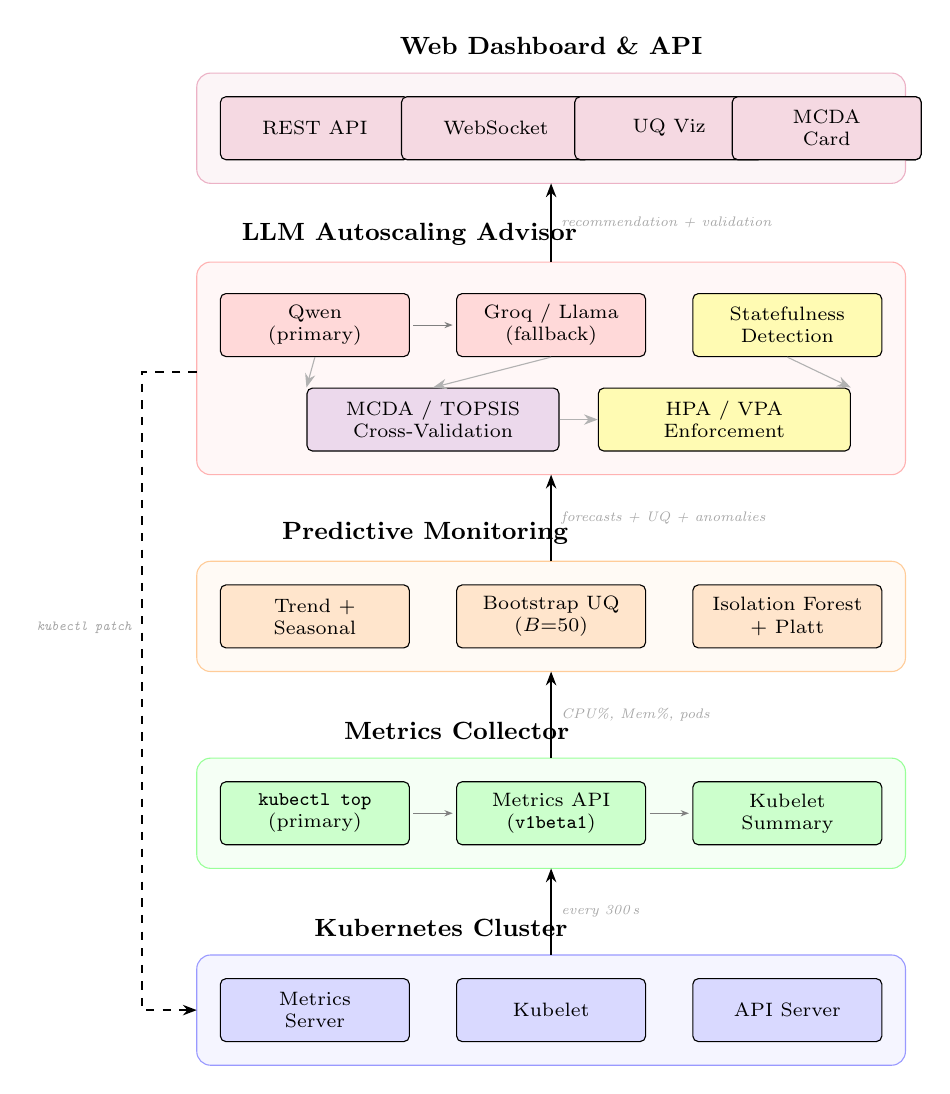
\begin{tikzpicture}[
    sub/.style={draw, rounded corners=2pt, fill=#1, font=\scriptsize,
                align=center, inner sep=3pt, minimum width=2.4cm,
                minimum height=0.8cm},
    sub/.default={gray!10},
    arrow/.style={-{Stealth[length=5pt]}, thick},
    note/.style={font=\tiny\itshape, text=gray!70},
    title/.style={font=\small\bfseries}
]

% ---- Row 1: Kubernetes Cluster ----
\node[sub=blue!15]  (msrv) at (0,0)    {Metrics\\Server};
\node[sub=blue!15]  (klet) at (3,0)    {Kubelet};
\node[sub=blue!15]  (apis) at (6,0)    {API Server};
\draw[rounded corners=5pt, fill=blue!4, draw=blue!40]
      (-1.5,-0.7) rectangle (7.5,0.7);
\node[title] at (1.6,1.05) {Kubernetes Cluster};
% redraw sub-nodes on top
\node[sub=blue!15]  at (0,0)    {Metrics\\Server};
\node[sub=blue!15]  at (3,0)    {Kubelet};
\node[sub=blue!15]  at (6,0)    {API Server};

% ---- Row 2: Metrics Collection ----
\node[sub=green!20] (ktop) at (0,2.5)  {\texttt{kubectl top}\\(primary)};
\node[sub=green!20] (mapi) at (3,2.5)  {Metrics API\\(\texttt{v1beta1})};
\node[sub=green!20] (ksum) at (6,2.5)  {Kubelet\\Summary};
\draw[rounded corners=5pt, fill=green!4, draw=green!40]
      (-1.5,1.8) rectangle (7.5,3.2);
\node[title] at (1.8,3.55) {Metrics Collector};
\node[sub=green!20] at (0,2.5)  {\texttt{kubectl top}\\(primary)};
\node[sub=green!20] at (3,2.5)  {Metrics API\\(\texttt{v1beta1})};
\node[sub=green!20] at (6,2.5)  {Kubelet\\Summary};
% fallback arrows
\draw[-{Stealth[length=3pt]}, thin, gray] (1.25,2.5) -- (1.75,2.5);
\draw[-{Stealth[length=3pt]}, thin, gray] (4.25,2.5) -- (4.75,2.5);

% ---- Row 3: Predictive Monitoring ----
\node[sub=orange!20] (fore) at (0,5)   {Trend +\\Seasonal};
\node[sub=orange!20] (uq)   at (3,5)   {Bootstrap UQ\\($B{=}50$)};
\node[sub=orange!20] (anom) at (6,5)   {Isolation Forest\\+ Platt};
\draw[rounded corners=5pt, fill=orange!4, draw=orange!40]
      (-1.5,4.3) rectangle (7.5,5.7);
\node[title] at (1.4,6.05) {Predictive Monitoring};
\node[sub=orange!20] at (0,5)   {Trend +\\Seasonal};
\node[sub=orange!20] at (3,5)   {Bootstrap UQ\\($B{=}50$)};
\node[sub=orange!20] at (6,5)   {Isolation Forest\\+ Platt};

% ---- Row 4: LLM Advisor (two sub-rows) ----
\draw[rounded corners=5pt, fill=red!3, draw=red!30]
      (-1.5,6.8) rectangle (7.5,9.5);
\node[title] at (1.2,9.85) {LLM Autoscaling Advisor};
% sub-row A: models + detection
\node[sub=red!15]    (qwen)  at (0,8.7)   {Qwen\\(primary)};
\node[sub=red!15]    (groq)  at (3,8.7)   {Groq / Llama\\(fallback)};
\node[sub=yellow!30] (sdet)  at (6,8.7)   {Statefulness\\Detection};
% sub-row B: MCDA + enforcement
\node[sub=violet!15, minimum width=3.2cm] (mcda) at (1.5,7.5)
      {MCDA / TOPSIS\\Cross-Validation};
\node[sub=yellow!30, minimum width=3.2cm] (enf)  at (5.2,7.5)
      {HPA / VPA\\Enforcement};
% fallback arrow
\draw[-{Stealth[length=3pt]}, thin, gray] (1.25,8.7) -- (1.75,8.7);
% internal flows
\draw[arrow, thin, gray!60] (qwen.south)  -- (mcda.north west);
\draw[arrow, thin, gray!60] (groq.south)  -- (mcda.north);
\draw[arrow, thin, gray!60] (sdet.south)  -- (enf.north east);
\draw[arrow, thin, gray!60] (mcda.east)   -- (enf.west);

% ---- Row 5: Dashboard ----
\node[sub=purple!15] (rest) at (0,11.2)    {REST API};
\node[sub=purple!15] (ws)   at (2.3,11.2)  {WebSocket};
\node[sub=purple!15] (uiv)  at (4.5,11.2)  {UQ Viz};
\node[sub=purple!15] (mcv)  at (6.5,11.2)  {MCDA\\Card};
\draw[rounded corners=5pt, fill=purple!4, draw=purple!30]
      (-1.5,10.5) rectangle (7.5,11.9);
\node[title] at (3,12.25) {Web Dashboard \& API};
\node[sub=purple!15] at (0,11.2)    {REST API};
\node[sub=purple!15] at (2.3,11.2)  {WebSocket};
\node[sub=purple!15] at (4.5,11.2)  {UQ Viz};
\node[sub=purple!15] at (6.5,11.2)  {MCDA\\Card};

% ---- Arrows between layers ----
\draw[arrow] (3,0.7)   -- node[right, note, pos=0.5] {every 300\,s} (3,1.8);
\draw[arrow] (3,3.2)   -- node[right, note, pos=0.5] {CPU\%, Mem\%, pods}
                           (3,4.3);
\draw[arrow] (3,5.7)   -- node[right, note, pos=0.5]
                           {forecasts + UQ + anomalies} (3,6.8);
\draw[arrow] (3,9.5)   -- node[right, note, pos=0.5]
                           {recommendation + validation} (3,10.5);

% ---- Actuation return arrow ----
\draw[arrow, dashed] (-1.5,8.1) -- (-2.2,8.1) |- node[left, note, pos=0.2]
      {\texttt{kubectl patch}} (-1.5,0);

\end{tikzpicture}
\Description{Detailed architecture of AutoSage with five layers, each
containing separate sub-component boxes.  Kubernetes Cluster has Metrics
Server, Kubelet, API Server.  Metrics Collection has three fallback methods
connected by arrows.  Predictive Monitoring has forecasting, bootstrap UQ,
and anomaly detection.  LLM Advisor has two rows: Qwen/Groq with
statefulness detection, and MCDA/TOPSIS with HPA/VPA enforcement, connected
by internal flow arrows.  Web Dashboard has REST, WebSocket, UQ Viz, MCDA
Card.  Layer arrows show data flow; dashed arrow shows actuation return.}
\caption{Architecture of \Solution{}.  Each layer contains its internal
components as separate modules.  Solid arrows show the data flow; the dashed
arrow shows the actuation path.  Small gray arrows within layers indicate
internal flows (e.g., \ LLM fallback chain, MCDA feeding enforcement). \as{In k8s cluster we miss kubelet top right?}} \pn{if you mean kubectl top then we should not put kubectl top inside the Kubernetes Cluster layer.kubectl top is a client command/tool (outside the cluster),it queries cluster metrics through the API path (Metrics Server / API Server),so it belongs to the Metrics Collection layer, not inside cluster internals.}
\label{fig:arch}
\end{figure*}

\subsection{Metrics Collector}
\label{sec:metrics}

The \emph{Metrics Collector} gathers real-time resource telemetry from the target K8s cluster.  Rather than requiring a full monitoring stack such as Prometheus, \Solution{} queries only a lightweight Kubernetes Metrics Server~\cite{}\as{add ref} \pn{i added them in bibliography but when i use them in cite the compile breaks!}, a scalable and efficient plugin that operates a source of container resource metrics for autoscaling pipelines.
In such a way, our approach works with any standard cluster, eliminating the need to deploy additional infrastructure.  
The collector retrieves metrics using a prioritized, sequential strategy. It first attempts to obtain metrics using a primary method. If this attempt fails or does not return within a fixed timeout ($10$\,s), the system proceeds to the next method in the predefined order. This process continues until metrics are successfully retrieved or all available methods have been attempted. 
%Each individual metrics request is allowed to run for at most 10\,s. 
Individual requests that exceed this timeout are treated as failed, triggering the next method in the sequence. This design ensures predictable latency while providing robustness against transient failures or slow responses from individual metric sources.

The collector attempts to retrieve metrics from the following sources, in order of priority:
\begin{enumerate}
    \item \textbf{Kubectl top.}  The primary method executes \texttt{kubectl top nodes} as a subprocess and parses the tabular output for per-node CPU (millicores) and memory (MiB).  This service internally reads from the Metrics Server but returns values in a format similar to the traditional \texttt{top} command. We have empirically observed that on a single-node testbed, this call completes in ${\sim}200$--$500$\,ms, which makes our timeout value a valid threshold.
    %\pn{In our single-node CrownLabs testbed, this call typically completed in a few hundred milliseconds (empirical observation).}
    \item \textbf{Metrics API.}  If \texttt{kubectl top} fails or is unavailable, the collector queries via direct API requests to the Metrics Server. The endpoint \texttt{metrics.\allowbreak{}k8s.\allowbreak{}io/v1beta1} is accessed via a Kubernetes Python client, %(\texttt{CustomObjectsApi}), 
    converting raw millicore and byte values to percentages using each node's allocatable capacity. 
    \item \textbf{Kubelet Summary API.}  As a last resort, the collector queries each node's Kubelet via the API server proxy that returns \texttt{usageNanoCores}. This value represents how much CPU a workload is using, thus we convert it to CPU usage using the formula 1\,CPU\,$=$\,$10^{9}$\,nanocores.
\end{enumerate}

The methods are not executed in parallel since only one method is active per collection cycle; the fallback is transparent to downstream consumers.  Raw values are normalized to cluster-wide utilization percentages: $\text{CPU\%} = \text{usage} / \text{allocatable} \times 100$, and analogously for memory.  
The \emph{Metrics Collector} generates an aggregated snapshot consisting of: CPU\%, memory\%, pod count \as{what is this? no explanation, not all are familiar with k8s} \pn{Pod count is the number of pods currently running for the monitored workload/namespace. It gives a direct view of how many application instances are active.}, node count \as{what is this? no explanation} \pn{Node count is the number of Kubernetes worker machines currently available in the cluster. It indicates cluster capacity and helps normalize resource usage.},
network~I/O \as{what is this? no explanation} \pn{Network I/O is the amount of data sent and received over the network by the monitored workloads/nodes (input/output traffic). It is useful to detect communication-heavy load conditions.}, and disk~I/O \as{what is this? no explanation} \pn{Disk I/O is the amount of data read from and written to storage by workloads/nodes. It captures storage pressure that may not appear in CPU or memory alone.}. With a time interval $\Delta t$, the module generates a matrix \as{Is it a matrix or array?} \pn{It is an array (list) of snapshots in the implementation.
You can think of it like a matrix when explaining it, but technically it is stored as a rolling list.}using the last $N$ samples in a rolling in-memory window to feed the forecasting module. By default, we set = $\Delta t =300$\,s but this value can be customized for faster or slower decisions.

\subsection{Predictive Monitoring}
\label{sec:prediction}

\subsubsection{Time-Series Forecasting.}
CPU utilization is forecast over a horizon of $H = 6$~hours using a composite model. A first-order polynomial (linear trend) is fitted to the last~$N$ samples via least-squares, %(\texttt{numpy.polyfit})
and a seasonal component capturing daily periodicity is added:
\begin{equation}\label{eq:forecast}
  \hat{y}(t+h) \;=\; 0.7 \cdot f_{\mathrm{trend}}(t+h)
                 \;+\; 0.3 \cdot f_{\mathrm{season}}(t+h),
  \quad h = 1, \ldots, H
\end{equation}
where $f_{\mathrm{trend}}$ is the linear extrapolation and $f_{\mathrm{season}}$ is the corresponding value from the previous daily cycle. \as{We need more explanation here. what is 0.7 and 0.3? How is this combined with least-squares?} \pn{0.7 and 0.3 are fixed blending weights.
First, least-squares is used to fit the linear trend term.
Then the final forecast is computed as a weighted sum:
70% from the trend model and 30% from the seasonal component.
So least-squares is used only to estimate the trend part, and then both parts are combined using those weights.}
Memory utilization is forecast with a separate exponential-smoothing model
($\alpha = 0.3$):
\begin{equation}\label{eq:mem_smoothing}
  \hat{m}_{t+1} = \alpha m_t + (1-\alpha)\hat{m}_{t},
\end{equation}
where $m_t$ is the observed memory utilization at time $t$ and $\hat{m}_t$ is
the smoothed estimate from the previous step. \as{is it a new formula or same as before?} \pn{It is a different formula (separate model). CPU uses the trend+seasonal equation in Eq.~\ref{eq:forecast}, while memory uses exponential smoothing in Eq.~\ref{eq:mem_smoothing}.}

\subsubsection{Bootstrap Uncertainty Quantification.}
\label{subsec:uncert}

Point forecasts alone cannot express how much trust an operator should place in
a prediction.  \Solution{} therefore wraps every forecast in a
\emph{prediction interval} produced by bootstrap resampling~\cite{efron1993introduction}.

Given $N$ historical observations, the forecaster draws $B = 50$ bootstrap
samples of size~$N$ with replacement.  For each resample~$b$, a linear model
is fitted and predictions $\hat{y}^{(b)}(t+h)$ are computed for each
horizon~$h$.  The epistemic (model) variance at horizon~$h$ is
\begin{equation}\label{eq:epistemic}
  \sigma^2_{\mathrm{epi}}(h) =
    \frac{1}{B}\sum_{b=1}^{B}
      \bigl(\hat{y}^{(b)}(t+h) - \bar{y}(t+h)\bigr)^{2},
\end{equation}
where $\bar{y}(t+h)$ is the mean bootstrap prediction.  The aleatoric (data
noise) variance $\sigma^2_{\mathrm{ale}}$ is estimated from the residuals of
the original fit.  The total variance grows with the forecast horizon:
\begin{equation}\label{eq:total_var}
  \sigma^2(h) = \sigma^2_{\mathrm{ale}} \cdot \sqrt{h}
              + \sigma^2_{\mathrm{epi}} \cdot h,
\end{equation}
yielding a $100(1{-}\alpha)\%$ prediction interval
$[\hat{y}(t{+}h) \pm z_{\alpha/2}\,\sigma(h)]$ (default 95\%, $z = 1.96$).
The system also computes four \emph{exceedance probabilities}
$\Pr\bigl[Y(t{+}h) > \tau\bigr]$ for thresholds
$\tau \in \{50, 70, 80, 90\}\%$ using the complementary normal CDF. \as{what is this? how is it used?}
\as{We need to expan a bit more here} \pn{The prediction interval gives a plausible range for future utilization (not just one point estimate).
Then, exceedance probability estimates how likely utilization is to cross practical thresholds (50/70/80/90%).
These probabilities are used by the dashboard and autoscaling logic: higher exceedance at high thresholds means higher risk and can trigger stronger scale-up recommendations, while low exceedance supports maintain/scale-down decisions. or we can say it like  this The interval \([\hat{y}(t+h)\pm z_{\alpha/2}\sigma(h)]\) provides the expected range of future utilization at confidence \(100(1-\alpha)\%\), so operators can see forecast uncertainty instead of only a point estimate. In addition, the system computes exceedance probabilities \(\Pr(Y(t+h)>\tau)\) for \(\tau\in\{50,70,80,90\}\%\). These values directly express operational risk (e.g., probability of entering high or critical utilization zones) and are used in both dashboard visualization and scaling decisions.}

\subsubsection{Calibrated Anomaly Detection.}
An Isolation Forest~\cite{liu2008isolation} with contamination
$c = 0.1$ produces a raw anomaly score $s \in [-1,1]$.  Since raw scores are
not directly interpretable as probabilities, \Solution{} applies
\emph{Platt scaling}~\cite{platt1999probabilistic}:
\begin{equation}\label{eq:platt}
  \Pr(\text{anomaly} \mid s) = \sigma(As + B)
    = \frac{1}{1 + e^{-(As + B)}},
\end{equation}
with learned parameters $A = -5.0$ and $B = -0.5$.  The calibrated probability
is mapped to a severity distribution across four levels (low, medium, high,
critical), and a detection confidence is computed as
$\gamma = 2 \, |P(\text{anomaly}) - 0.5|$. \as{what is this? how is it used?} \as{We need to expan a bit more here} \pn{This block converts anomaly detection from a binary flag into a risk score that operators can act on.
Isolation Forest gives a raw anomaly score, but raw scores are hard to interpret.
Platt scaling transforms that score into an estimated probability of anomaly (0 to 1), which is easier to understand and compare over time.
That probability is then mapped to severity levels (low/medium/high/critical) for dashboard display and alert prioritization.
The confidence term 
γ=2∣P(anomaly)−0.5∣ γ=2∣P(anomaly)−0.5∣ measures how far the probability is from uncertainty (0.5): values near 1 mean strong confidence, values near 0 mean uncertain detection.
In practice, these outputs are used to trigger warnings, explain risk in the UI, and provide additional context to scaling decisions.”
}

\subsection{LLM Autoscaling Advisor}
\label{sec:llm}

The autoscaling advisor casts every scaling decision as a natural-language
reasoning problem.  A structured prompt is assembled from four sources of
context: (i)~current metrics (CPU/memory utilisation, pod count,
ready/available pods), (ii)~forecasts (current value, peak, trend, per-hour
predictions for $H = 6$~hours), (iii)~deployment state (replicas, min/max
bounds, resource requests/limits, HPA/VPA status), and (iv)~statefulness
classification (see below).  The LLM returns a JSON object specifying the
recommended \texttt{action} (\texttt{scale\_up}, \texttt{scale\_down}, or
\texttt{maintain}), a \texttt{scaling\_type} (\texttt{hpa} or \texttt{vpa}),
target replicas or VPA resource requests, a confidence score, and a free-text
rationale.

\subsubsection{Model Selection and Caching.}
\Solution{} implements a two-tier LLM fallback chain.  The primary model is a
self-hosted open-source LLM (e.g.\ Qwen) accessed via an OpenAI-compatible
endpoint, with a timeout of 240\,s and generation temperature $\theta = 0.1$.
If the primary model is unavailable, the system falls back to the Groq cloud
API (Llama~3.1-8B, timeout 15\,s).  To limit API costs, recommendations are
cached for a configurable TTL (default 300\,s) and calls are rate-limited to a
minimum interval of 30\,s.

\subsubsection{HPA vs.\ VPA Decision.}\label{sec:hpa-vpa}
Choosing between horizontal and vertical scaling is fundamental: adding
replicas (HPA) to a stateful application that stores session data inside the
pod would cause data loss, while increasing per-pod resources (VPA) for a
stateless web server wastes capacity that could be spread across replicas.
\Solution{} determines the scaling type through a three-stage process.

\paragraph{Stage~1: Statefulness Detection.}
Before calling the LLM, the system inspects the Kubernetes deployment object
and classifies the workload's state management through five signals, evaluated
in priority order:
\begin{enumerate}
  \item \textbf{Annotation}
        (\texttt{ai4k8s.io/\allowbreak{}state\--management}):
        explicit operator declaration (\emph{high} confidence).
  \item \textbf{Environment variables}: presence of \texttt{REDIS},
        \texttt{DATABASE}, \texttt{POSTGRES} indicates stateless (external
        state); \texttt{LOCAL\_STORAGE}, \texttt{PERSISTENT} indicates
        stateful (\emph{medium} confidence).
  \item \textbf{Persistent volumes}:
        \texttt{PersistentVolumeClaim} or \texttt{hostPath} mounts indicate
        stateful (\emph{high} confidence); \texttt{emptyDir} is ignored.
  \item \textbf{Namespace services}: presence of Redis, database, or cache
        services in the same namespace indicates stateless (\emph{medium}).
  \item \textbf{Labels}: standard Kubernetes labels provide additional hints
        (\emph{low} confidence).
\end{enumerate}
The detected type and confidence are included in the LLM prompt.

\paragraph{Stage~2: LLM Reasoning.}
The LLM receives the statefulness classification as part of the prompt and
returns a \texttt{scaling\_type} field.  Because the LLM has access to the full
deployment context, it can make nuanced decisions---for example, recommending
VPA when a stateless application is already at maximum replicas.

\paragraph{Stage~3: Post-Processing Enforcement.}
LLM outputs can be inconsistent: the reasoning text may mention ``state stored
inside the pod'' while the JSON sets \texttt{scaling\_type:~hpa}.  A
rule-based enforcement layer catches such contradictions:
\begin{itemize}
  \item If the reasoning contains stateful indicators but the output is HPA, the system corrects to VPA and computes the target CPU/memory from the current usage plus a 20\% headroom.
  \item If the detection classifies the workload as stateless but the LLM outputs VPA, the system forces HPA and recalculates target replicas from current metrics and forecast peaks.
  \item If no statefulness information is available and the LLM chose HPA,
        the system defaults to VPA as the safer option.
\end{itemize}

\subsubsection{Scaling Actuation.}
Once the scaling type and targets are finalised, the corresponding engine module applies the change:
\begin{itemize}
  \item \textbf{HPA:} a JSON Patch sets \texttt{minReplicas} and
        \texttt{maxReplicas} on the HPA resource
        (\texttt{kubectl patch hpa --type=json}).
  \item \textbf{VPA:} a strategic merge patch updates the container's \\
        \texttt{resources.requests} in the Deployment spec
        (\texttt{kubectl patch deployment --type=merge}).
\end{itemize}

\subsection{MCDA Cross-Validation}\label{sec:mcda}

LLM recommendations are inherently non-deterministic.  To provide a formal safeguard, every recommendation is cross-validated by a Multi-Criteria Decision Analysis (MCDA) module that implements the Technique for Order of Preference by Similarity to Ideal Solution (TOPSIS)~\cite{hwang1981topsis}.

\subsubsection{Alternative Generation.}
From the current replica count~$r$, the module generates $5$--$8$ candidate
alternatives: $r + \delta$ for $\delta \in \{-2, -1, 0, +1, +2, +3\}$, the
minimum and maximum replicas, and an ``ideal'' replica count that would bring
CPU utilisation to~70\%.  Candidates outside the $[\textit{min},\textit{max}]$
range are discarded.

\subsubsection{Criteria Evaluation.}
Each alternative is scored on five criteria (Table~\ref{tab:criteria}).  Scores
are normalised, weighted, and processed by the TOPSIS algorithm.

\begin{table}[t]
\caption{MCDA criteria and their evaluation.}
\label{tab:criteria}
\centering
\small
\begin{tabular}{@{}llp{3.8cm}@{}}
\toprule
\textbf{Criterion} & \textbf{Type} & \textbf{Description} \\
\midrule
Cost            & Cost    & Normalised replica count $r / r_{\max}$ \\
Performance     & Benefit & Proximity of estimated CPU to 70\% sweet spot \\
Stability       & Benefit & Penalises large replica changes and contra-trend scaling \\
Forecast Align. & Benefit & Estimated peak CPU in 50--75\% comfort zone \\
Response Time   & Cost    & Estimated CPU as proxy for latency \\
\bottomrule
\end{tabular}
\end{table}

\subsubsection{TOPSIS Ranking.}
Let $\mathbf{X} \in \mathbb{R}^{m \times n}$ be the decision matrix with $m$
alternatives and $n = 5$ criteria.  TOPSIS proceeds as follows:
\begin{enumerate}
  \item \textbf{Normalise:}
        $r_{ij} = x_{ij} \big/ \sqrt{\sum_{i=1}^{m} x_{ij}^2}$.
  \item \textbf{Weight:}
        $v_{ij} = w_j \cdot r_{ij}$, where $\mathbf{w}$ is one of four
        predefined weight profiles (balanced, performance-first,
        cost-optimised, stability-first).
  \item \textbf{Ideal / Anti-ideal:}
        $A^{+}_j = \max_i v_{ij}$ (benefit) or $\min_i v_{ij}$ (cost);
        $A^{-}_j$ vice versa.
  \item \textbf{Distances:}
        $D^{+}_i = \lVert \mathbf{v}_i - A^{+} \rVert_2$, \;
        $D^{-}_i = \lVert \mathbf{v}_i - A^{-} \rVert_2$.
  \item \textbf{Closeness:}
        $C_i = D^{-}_i / (D^{+}_i + D^{-}_i) \in [0,1]$.
\end{enumerate}
The alternative with the highest $C_i$ is the MCDA-optimal action.

\subsubsection{Agreement and Override.}
The MCDA module compares the LLM's recommended target~$r_L$ with the
MCDA-optimal target~$r_M$.  Agreement is classified into three levels:
\begin{itemize}
  \item \textbf{Full agreement:} same scaling direction and
        $|r_L - r_M| \leq 1$.
  \item \textbf{Partial agreement:} same direction, different magnitude.
  \item \textbf{Divergence:} opposite scaling directions.
\end{itemize}
If partial or divergent and the MCDA closeness score exceeds the LLM's by more
than a threshold $\delta = 0.15$, the system overrides the LLM recommendation
with the MCDA-optimal action.  The full validation result---agreement level,
both scores, the dominance margin, criteria weights, and ranking---is attached
to the recommendation and displayed on the dashboard.

\subsubsection{Weight Profiles.}
Four weight profiles allow operators to express different priorities
(Table~\ref{tab:weights}).  The default profile is \emph{balanced}.

\begin{table}[t]
\caption{MCDA weight profiles ($w_j$ sums to 1.0).}
\label{tab:weights}
\centering
\small
\begin{tabular}{@{}lccccc@{}}
\toprule
\textbf{Profile} & \textbf{Cost} & \textbf{Perf.} & \textbf{Stab.}
                  & \textbf{Forec.} & \textbf{Resp.} \\
\midrule
Balanced           & 0.20 & 0.30 & 0.25 & 0.15 & 0.10 \\
Performance-first  & 0.10 & 0.40 & 0.15 & 0.20 & 0.15 \\
Cost-optimised     & 0.40 & 0.20 & 0.20 & 0.10 & 0.10 \\
Stability-first    & 0.15 & 0.20 & 0.40 & 0.15 & 0.10 \\
\bottomrule
\end{tabular}
\end{table}

\subsection{Dashboard and Actuation}\label{sec:dashboard}

% \Solution{} exposes a Flask-based web application that serves both REST
% endpoints and WebSocket channels (via Flask-SocketIO).  The monitoring
% dashboard renders:
% \begin{itemize}
%   \item Prediction intervals that widen with the forecast horizon, providing a
%         visual cue of uncertainty growth.
%   \item Exceedance probability bars for four utilization thresholds.
%   \item Stacked bars decomposing total uncertainty into aleatoric and
%         epistemic components.
%   \item Calibrated anomaly probability with severity distribution.
%   \item MCDA validation cards showing agreement level, TOPSIS scores, and
%         ranking.
% \end{itemize}
% Scaling recommendations are generated asynchronously; the frontend polls via
% WebSocket for status updates and displays a progress indicator.  When an
% operator approves a recommendation, the dashboard triggers a
% \texttt{kubectl~patch} command through the appropriate engine module
% (\texttt{autoscaling\_engine} for HPA, \texttt{vpa\_engine} for VPA), closing
% the actuation loop.

\Solution{} exposes a web-based control plane that provides both REST APIs and WebSocket channels for real-time interaction via Flask and Flask-SocketIO. The monitoring dashboard presents: \textit{(i)} prediction intervals that expand with the forecast horizon to reflect uncertainty growth; \textit{(ii)} the four exceedance probabilities across the utilization thresholds $(50, 70, 80, 90)$ as mentioned in Section~\ref{subsec:uncert}; 
% because the system computes probabilities for thresholds 50 70 80 90 percent they are defined earlier in the predictive/UQ part.
\textit{(iii)} where prediction uncertainty comes from (data noise vs model uncertainty), in the form a decomposition of predictive uncertainty into aleatoric (Eq.(\ref{eq:total_var})) \as{not sure if this is the right eq} and epistemic (Eq.(\ref{eq:epistemic})) components; 
\textit{(iv)} calibrated anomaly likelihood with associated severity; 
and \textit{(v)} MCDA-based validation summaries including agreement levels, TOPSIS scores, and ranking.

Scaling recommendations are computed asynchronously and streamed to the frontend with progress updates. Upon operator approval, the system actuates the selected policy (via \texttt{kubectl~patch} command) by invoking the appropriate autoscaling module (HPA or VPA), thereby closing the monitoring–analysis–decision–actuation loop.

\section{Evaluation}
\label{sec:evaluation}

This section reports a live comparison between Kubernetes-native autoscaling
and \Solution{}, with emphasis on timing, service-level behavior, and resource
footprint under the same workload conditions.

\subsection{Comparison with Native HPA/VPA}

To quantify the practical behavior of \Solution{} against Kubernetes-native
autoscalers, we implemented and executed a dedicated benchmark runner
(\texttt{autoscaling\_native\_comparison.py}) in the project repository. The
runner now supports repeated experiments (\texttt{--runs}, default \(N=10\)),
and reports mean, standard deviation, and 95\% confidence intervals for each
metric. The experiment was run on the CrownLabs deployment used throughout this
work, on the \texttt{test-app-autoscaling} workload in namespace
\texttt{ai4k8s-test}. For fairness, each method starts from the same baseline
(\(2\) replicas) before load is applied.

Load was generated in two ways: (i) increasing background CPU pressure by
setting \texttt{CPU\_LOAD\_PERCENT=95} in the target deployment, and
(ii) issuing burst requests to \texttt{/cpu-load} from an ephemeral in-cluster
\texttt{curl} pod. Three strategies were then evaluated with a per-method
timeout of \(60\) seconds: native HPA, native VPA, and \Solution{} predictive
autoscaling (LLM + MCDA + actuation). To make timing semantics explicit, we
separate three phases in the loop: (1) \emph{control-plane provisioning}
(object create/update latency in the API server), (2) \emph{decision/reaction}
(time until a scaling recommendation or controller decision appears), and
(3) \emph{post-decision actuation} (time from decision availability to first
applied resource change). The repeated-run protocol also includes warm-up,
cool-down, and cleanup checks between methods to improve reproducibility.

\begin{table}[t]
  \centering
  \caption{Live CrownLabs comparison: native HPA/VPA vs. \Solution{} (latest run example).}
  \label{tab:native-compare}
  \footnotesize
  \setlength{\tabcolsep}{3pt}
  \renewcommand{\arraystretch}{1.1}
  \begin{tabular}{>{\raggedright\arraybackslash}p{1.2cm}
                  >{\raggedright\arraybackslash}p{1.45cm}
                  >{\raggedright\arraybackslash}p{2.15cm}
                  >{\raggedright\arraybackslash}p{2.55cm}}
    \toprule
    Method & Provisioning & Decision/Reaction & Outcome \\

    \midrule
    Native HPA & 0.198\,s & 31.288\,s to first scale-up & \(2 \rightarrow 6\) \\
    Native VPA & 0.478\,s & 0.180\,s to first recommendation & Recommendation produced \\
    \Solution{} & N/A & 111.789\,s to recommendation & \(2 \rightarrow 5\); first change at 0.302\,s \\
    \bottomrule
  \end{tabular}
\end{table}

\begin{table}[t]
  \centering
  \caption{Service-level and cost-proxy metrics (latest run example; aggregated statistics are reported as mean \(\pm\) 95\% CI in the JSON output).}
  \label{tab:service-cost}
  \footnotesize
  \setlength{\tabcolsep}{3pt}
  \renewcommand{\arraystretch}{1.1}
  \begin{tabular}{>{\raggedright\arraybackslash}p{1.65cm}
                  >{\raggedleft\arraybackslash}p{1.15cm}
                  >{\raggedleft\arraybackslash}p{1.15cm}
                  >{\raggedleft\arraybackslash}p{1.55cm}}
    \toprule
    Method & p95 latency (s) & SLA viol. (\%) & Cost proxy (avg req. vCPU) \\
    \midrule
    Native HPA & 0.0316 & 0.0 & 2.828 \\
    Native VPA & 0.0442 & 0.0 & 1.414 \\
    \Solution{} & 0.0313 & 0.0 & 3.535 \\
    \bottomrule
  \end{tabular}
\end{table}
\begin{figure}[t]
  \centering
  \IfFileExists{figures/evaluation/evaluation_decision_latency.pdf}
    {\includegraphics[width=\columnwidth]{figures/evaluation/evaluation_decision_latency.pdf}}
    {\fbox{\parbox{0.95\columnwidth}{\centering Missing file:\\ figures/evaluation/evaluation\_decision\_latency.pdf}}}
  \caption{Decision/reaction latency across native HPA, native VPA, and \Solution{} (error bars show 95\% CI when repeated-run aggregated data is provided).}
  \label{fig:evaluation-decision}
\end{figure}

\begin{figure}[t]
  \centering
  \IfFileExists{figures/evaluation/evaluation_service_levels.pdf}
    {\includegraphics[width=\columnwidth]{figures/evaluation/evaluation_service_levels.pdf}}
    {\fbox{\parbox{0.95\columnwidth}{\centering Missing file:\\ figures/evaluation/evaluation\_service\_levels.pdf}}}
  \caption{Service-level metrics (p95 latency and SLA violation rate); error bars show 95\% CI when available from repeated runs.}
  \label{fig:evaluation-service}
\end{figure}

\begin{figure}[t]
  \centering
  \IfFileExists{figures/evaluation/evaluation_cost_proxy.pdf}
    {\includegraphics[width=\columnwidth]{figures/evaluation/evaluation_cost_proxy.pdf}}
    {\fbox{\parbox{0.95\columnwidth}{\centering Missing file:\\ figures/evaluation/evaluation\_cost\_proxy.pdf}}}
  \caption{Cost proxy comparison using average requested vCPU during the evaluation window (95\% CI shown when repeated-run aggregation is available).}
  \label{fig:evaluation-cost}
\end{figure}

The results indicate a clear trade-off. Native controllers react faster in this
short-horizon setup, while \Solution{} adds decision latency due to LLM
inference and MCDA validation in the control loop. At the same time,
service-level behavior remains stable in the tested conditions, with low
request-path latency and no observed SLA violations in the sampled run.

For repeated runs, we interpret each metric through mean and 95\% confidence
interval rather than single-point values. In particular, CI overlap/non-overlap
is used as an uncertainty-aware indicator of whether observed differences are
likely robust across repetitions. This avoids over-interpreting one-off
executions and improves the scientific validity of the comparison.

Finally, cost is reported here as a \emph{resource proxy} (average requested
vCPU over sampled replicas), not direct cloud billing. The values therefore
represent relative footprint under the tested run rather than monetary cost.

\subsubsection{Evaluation Scope and Limitations}
The presented comparison should be interpreted as an ongoing evaluation
pipeline. Three limitations remain important for correct interpretation:
\textit{(i)} repeated trials and CI-based summaries must be generated and
reported for each benchmark campaign, \textit{(ii)} the reported cost is a
resource-based proxy rather than provider billing data, and
\textit{(iii)} short-horizon scenarios do not fully stress periodic/anticipatory
benefits of predictive autoscaling. A more complete study includes longer load
profiles with recurring bursts and explicit decomposition of LLM inference time,
MCDA processing time, and Kubernetes reconciliation time.

\section{Conclusion}
\label{sec:conclusion}

\bibliographystyle{ACM-Reference-Format}
\bibliography{bibliography}

\end{document}
